% Allow relative paths in included subfiles that are compiled separately
% See https://tex.stackexchange.com/questions/153312/
\providecommand{\main}{..}
\documentclass[\main/thesis.tex]{subfiles}

\begin{document}

% \chapter{Multilabel 12-Lead Electrocardiogram Classification Using Gradient Boosting Tree Ensemble}
\chapter{Joint Autoencoder Gradient Boosting Tree Ensemble}
\chaptermark{AENCXGB}
\label{chp:aencxgb}

In Chapter~\ref{chp:dl_autoenc} I discover that the autoencoder classification models provide worse overall challenge metrics compared to the gradient boosted tree model proposed in Chapter~\ref{chp:xgbensemble}, but are more sensitive in detecting \gls{irbbb}, \gls{lanfb}, and \gls{rad}.

This chapter explores the effectiveness of combining the autoencoder learned embeddings with the manually engineered features to train a new set of gradient boosted tree models.
I extend the approaches used in Chapters~\ref{chp:xgbensemble} and \ref{chp:dl_autoenc} with the following research questions:
\begin{itemize}
    \item For the shallow classification ensemble using manual feature engineering, the top $1,000$ features used were averaged across all classifier labels. Will selecting top features with respect to the label-wise classifier improve classification scoring metrics?
    \item We have a deep learning approach for generating a fixed size embedding representation of a variable length \gls{ecg} record. Will incorporating the sequence embeddings from our deep learning autoencoder improve classification scoring metrics?
    \item What are the new distributions of important feature categories for these new classifiers, with respect to each diagnosis?
\end{itemize}

% Unlike the prior two chapters, the work showcased in this chapter has not been published nor submitted for consideration.
% I acknowledge Dr. Sunil Vasu Kalmady for suggesting the idea of combining my two prior experiments together.
% All other facets are contributed by myself, as I engineered the experiment, generated the relevant figures, and wrote this writeup.

% The takeaways from this chapter are:
% \begin{enumerate}
%     \item Joining the autoencoder embeddings with the manually engineered features to train a set of gradient boosting tree ensemble classifiers resulted in models with poorer classification metrics than using manually engineered features alone.
%     \item Certain labels had increased mean classification $\text{F}_1$ score but none of the label-wise improvements were statistically significant at $p = 0.01$.
%     \item Long term viability of this strategy of combining deep learning techniques with shallow models is not promising, with notable disadvantages: no end-to-end training, unclear model interpretability.
% \end{enumerate}

% \section{Methodology}
% We extend the experiments performed in the manual feature engineering methodology~\cite{wong2020CINC-multilabel-ECG} discussed in Chapter~\ref{chp:xgbensemble} as well as the deep learning approach using the beat to sequence autoencoders~\cite{wong2021ICASSP-multilabel-ECG} discussed in Chapter~\ref{chp:dl_autoenc}.

% We run our corpus of available \gls{ecg} data through the manual feature engineering process to clean and pre-process our signals, then we extract the top 1,000 full waveform, heartbeat template, and heart rate variability features using \emph{tsfresh} and \emph{NeroKit2}.
% Additionally, using the 20 existing and trained beat to sequence autoencoders, we convert our \gls{ecg} records into embeddings of size 768 floating point numbers.
% Our classifier receives \gls{ecg} records as input vectors of size $1,768$.

% We use 20 times repeated random subsampling, keeping identical splits of our \gls{ecg} records as performed in our prior experiments, to mitigate internal validity risk.
% All other XGBoost configuration settings are identical to our previous XGBoost ensemble training experiment, which is discussed in Section~\ref{ssec:xgb_classification}.

% \section{Results}

% \begin{figure}[ht]
%     \centering
%     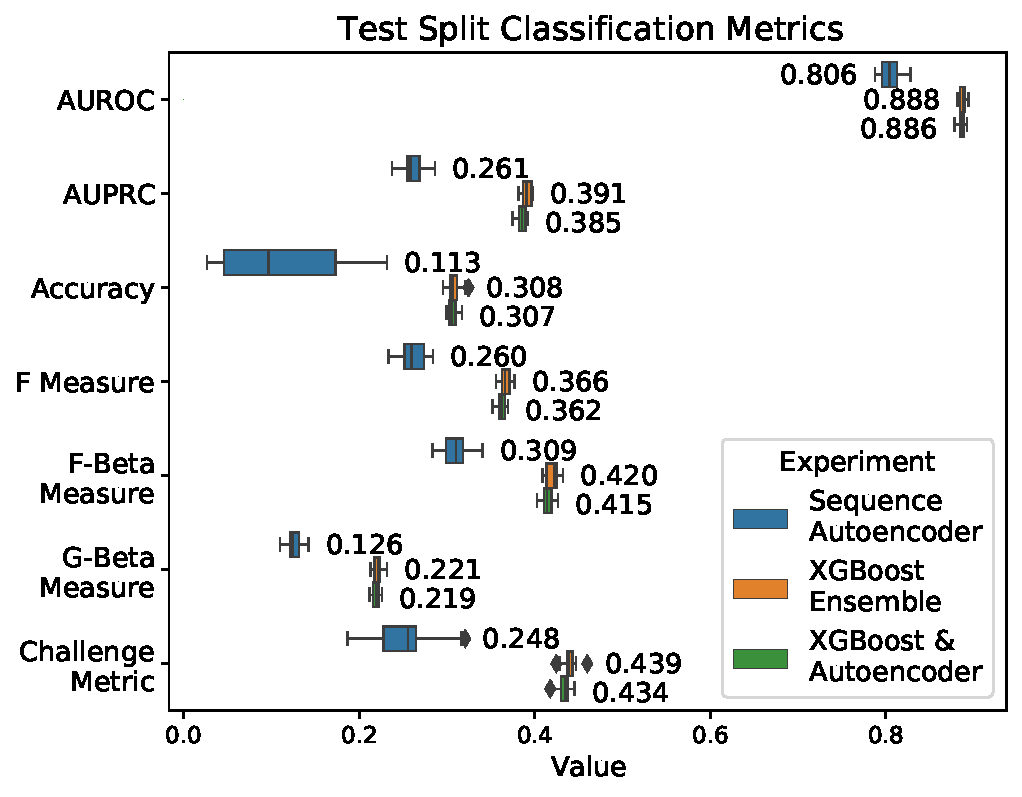
\includegraphics[width=10cm]{figure/classification_metrics_3_way.pdf}
%     \caption[Summary classification metrics comparing gradient boosting decision tree with manual feature engineering, beat to sequence autoencoder classifier, and gradient boosting decision tree with manual feature engineering and autoencoder embeddings.]{Summary classification metrics comparing gradient boosting decision tree with manual feature engineering, beat to sequence autoencoder classifier, and gradient boosting decision tree with manual feature engineering and autoencoder embeddings. Annotations indicate mean value.}
%     \label{fig:joint_xgb_aenc_classification_metrics_summary}
% \end{figure}

% Figure~\ref{fig:joint_xgb_aenc_classification_metrics_summary} contains the summary classification metrics of our original XGBoost methodology~\cite{wong2020CINC-multilabel-ECG}, our beat to sequence autoencoder~\cite{wong2021ICASSP-multilabel-ECG}, and the work discussed in this chapter joining these two approaches together.
% We observe that the additional features derived from the autoencoder caused all classification metrics to decrease respective to using the XGBoost ensemble methodology with manually engineered features alone.

% \begin{figure}[ht]
%     \centering
%     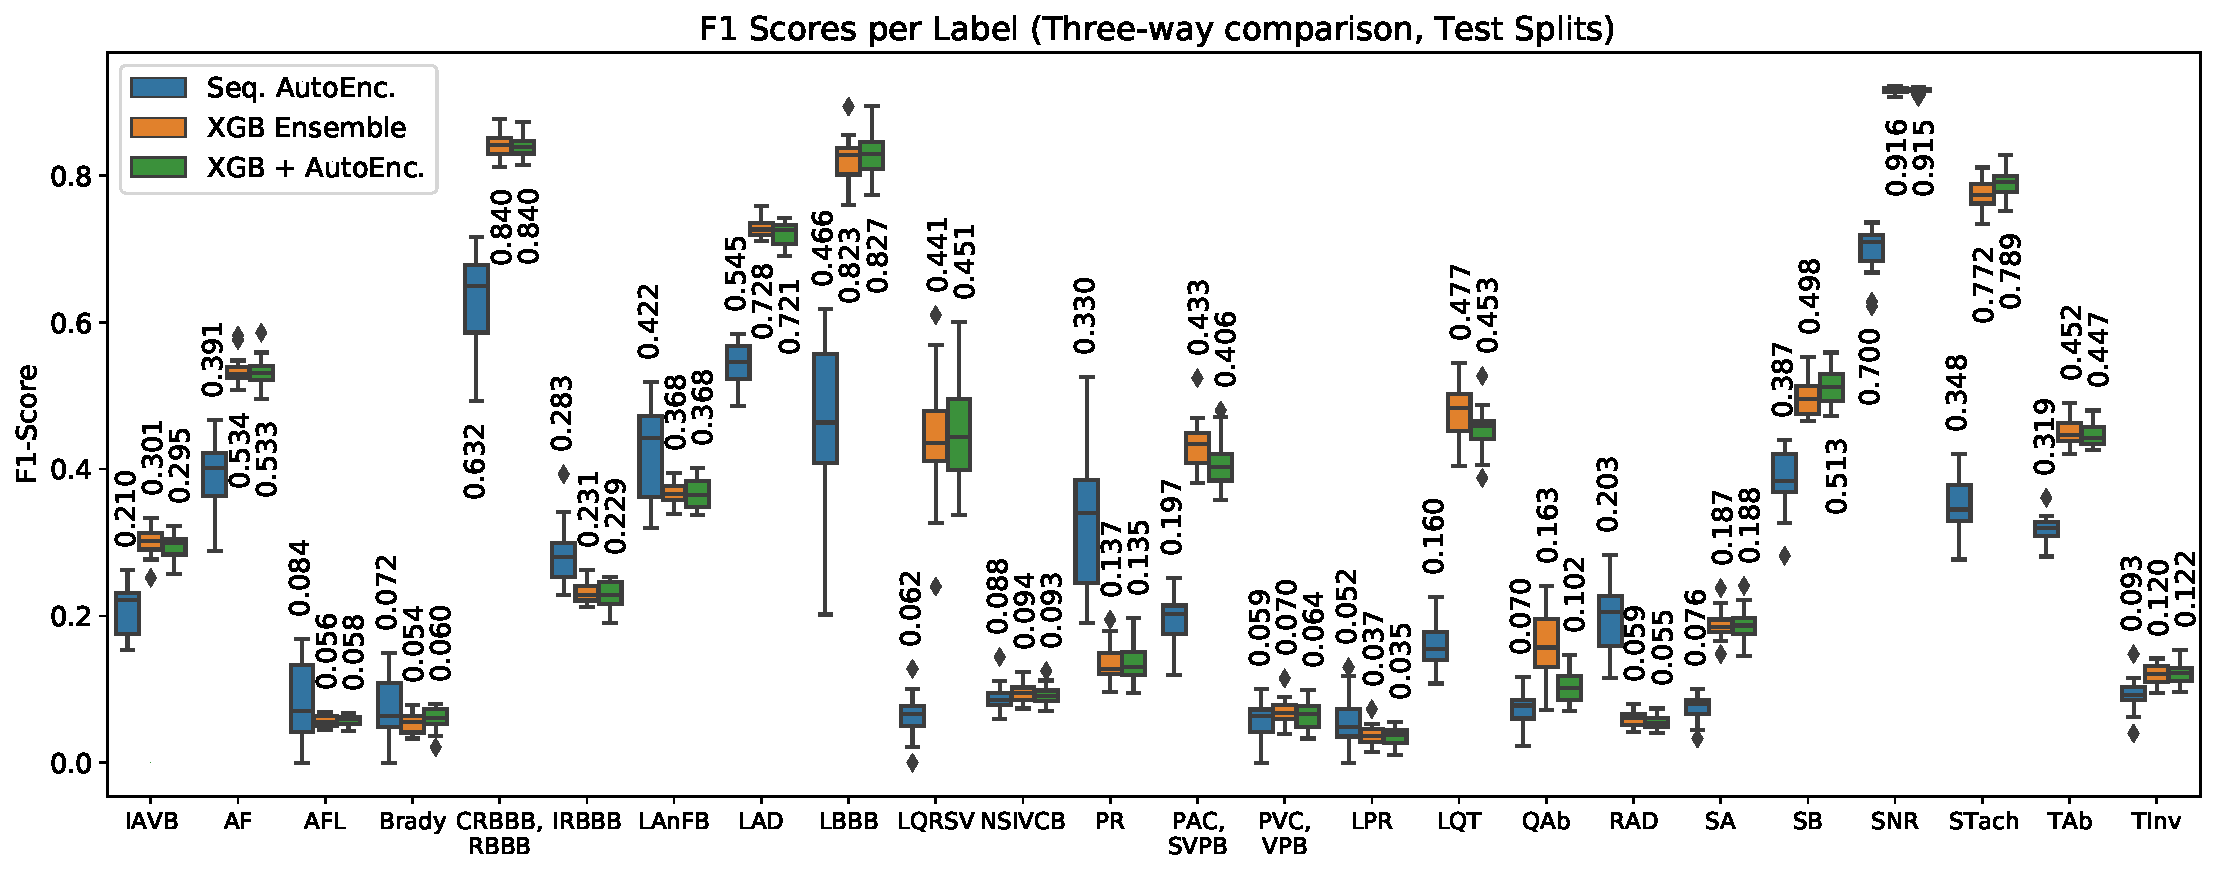
\includegraphics[width=14cm]{figure/label_f1s_3_way.pdf}
%     \caption[Label-wise $\text{F}_1$ scores comparing gradient boosting decision tree with manual feature engineering, beat to sequence autoencoder classifier, and gradient boosting decision tree with manual feature engineering and autoencoder embeddings.]{Label-wise $\text{F}_1$ scores comparing gradient boosting decision tree with manual feature engineering, beat to sequence autoencoder classifier, and gradient boosting decision tree with manual feature engineering and autoencoder embeddings. Annotations indicate mean value.}
%     \label{fig:joint_xgb_aenc_f1_score}
% \end{figure}

% A label-wise comparison of the joint model's $\text{F}_1$ scores compared to our prior work can be found in Figure~\ref{fig:joint_xgb_aenc_f1_score}.
% The Wilcoxon signed rank statistical test is used to compare the XGBoost with autoencoder embedding $\text{F}_1$ scores to the XGBoost without embedding $\text{F}_1$ scores.
% With a $p$-value of $0.01$, none of the labels incurred a statistically significant improvement in $\text{F}_1$ score.

% \section{Discussion}
% In a 2020 panel where Yoshua Bengio discusses current and upcoming deep learning challenges, he dismisses the viability of engineering deep learning models into old-fashioned symbolic machine learning methods, instead proposing learned attention mechanisms as a viable alternative~\cite{2020-yoshua-dlc}.

\end{document}
